\section{Algorithmus}

\begin{frame}
\frametitle{Algorithmus} 
\end{frame}

\newcommand{\dunderline}[1]{\underline{\underline{#1}}}
\subsection{Matrixumformung}
\begin{frame}
\begin{itemize}[<+->]
	\item $\dunderline{A}\cdot \dunderline{X} \ne \dunderline{f} \qquad\Rightarrow\qquad \dunderline{A}\cdot \underline{x} = \underline{f}$
	\item Matrix $f$
	\item Matrix $A$
\end{itemize}


\end{frame}
\subsection{Matrix A}
\begin{frame}

\tiny
\[
	A=\left(
	\begin{array}{ccccc|ccccc|c|ccccc}
	    -4&     1&     0&\cdots&     0 &     1&     0&     0&\cdots&     0 &\cdots &      &      &      &      &      \\
	     1&    -4&     1&\cdots&     0 &     0&     1&     0&\cdots&     0 &\cdots &      &      &      &      &      \\
	     0&     1&    -4&\cdots&     0 &     0&     0&     1&\cdots&     0 &\cdots &      &      &     0&      &      \\
	\vdots&\vdots&\vdots&\ddots&\vdots &\vdots&\vdots&\vdots&\ddots&\vdots &       &      &      &      &      &      \\
	     0&     0&     0&\cdots&    -4 &     0&     0&     0&\dots &     1 &\cdots &      &      &      &      &      \\
	\hline
	     1&     0&     0&\cdots&     0 &    -4&     1&     0&\dots &     0 &\cdots &      &      &      &      &      \\
	     0&     1&     0&\cdots&     0 &     1&    -4&     1&\dots &     0 &\cdots &      &      &      &      &      \\
	     0&     0&     1&\cdots&     0 &     0&     1&    -4&\dots &     0 &\cdots &      &      &     0&      &      \\
	\vdots&\vdots&\vdots&\ddots&\vdots &\vdots&\vdots&\vdots&\ddots&\vdots &       &      &      &      &      &      \\
	     0&     0&     0&\cdots&     1 &     0&     0&     0&\cdots&    -4 &\cdots &      &      &      &      &      \\
	\hline
	\vdots&\vdots&\vdots&      &\vdots &\vdots&\vdots&\vdots&      &\vdots &\ddots &\vdots&\vdots&\vdots&      &\vdots\\
	\hline
	      &      &      &      &       &      &      &      &      &       &\cdots &    -4&     1&     0&\cdots&     0\\
	      &      &      &      &       &      &      &      &      &       &\cdots &     1&    -4&     1&\cdots&     0\\
	      &      &     0&      &       &      &      &     0&      &       &\cdots &     0&     1&    -4&\cdots&     0\\
	      &      &      &      &       &      &      &      &      &       &       &\vdots&\vdots&\vdots&\ddots&\vdots\\
	      &      &      &      &       &      &      &      &      &       &\cdots &     0&     0&     0&\cdots&    -4\\
	\end{array}
	\right) 
	\]

\end{frame}

\subsection{Beispiel}
\begin{frame}
%\changefont{cmr}{m}{sl}

\tiny\centering
	$	A = \left(
	\begin{array}{ccc|ccc|ccc}
		-4 & 1 & 0  &  1 & 0 & 0 & 0 & 0 & 0 \\
		 1 &-4 & 1  &  0 & 1 & 0 & 0 & 0 & 0 \\
		 0 & 1 & -4 &  1 & 0 & 1 & 0 & 0 & 0 \\\hline
		 1 & 0 & 0  & -4 & 1 & 0 & 1 & 0 & 0 \\
		 0 & 1 & 0  & 1 & -4 & 1 & 0 & 1 & 0 \\
		 0 & 0 & 1  & 0 & 1 & -4 & 0 & 0 & 1 \\\hline
		 0 & 0 & 0  & 1 & 0 & 0 & -4 & 1 & 0 \\
		 0 & 0 & 0  & 0 & 1 & 0 & 1 & -4 & 1 \\
		 0 & 0 & 0  & 0 & 0 & 1 & 0 & 1 & -4 \\
	\end{array}
	\right)
	$
	
	\vspace{3em}
	
	$f = \left(
	\begin{array}{ccc}
		f_{11} & f_{12} & f_{13} \\
		f_{21} & f_{22} & f_{23} \\
		f_{31} & f_{32} & f_{33} 
	\end{array}
	\right) \quad\Rightarrow\quad
	f = \left(
	\begin{array}{c}
		f_{11} \\
		f_{21}\\
		f_{31}\\
		f_{12}\\
		f_{22}\\
		f_{32}\\
		f_{13}\\
		f_{23}\\
		f_{33}
	\end{array}
	\right)$
	\hspace{3em}
	$x = \left(
	\begin{array}{ccc}
		x_{11} & x_{12} & x_{13} \\
		x_{21} & x_{22} & x_{23} \\
		x_{31} & x_{32} & x_{33} 
	\end{array}
	\right) \quad\Rightarrow\quad
	x = \left(
	\begin{array}{c}
		x_{11} \\
		x_{21}\\
		x_{31}\\
		x_{12}\\
		x_{22}\\
		x_{32}\\
		x_{13}\\
		x_{23}\\
		x_{33}
	\end{array}
	\right)$
	
	\scriptsize
	\vspace{3em}
	$f_{ij}= x_{i(j-1)} + x_{i(j+1)} + x_{(i-1)j} + x_{(i+1)j}- 4\cdot x_{ij}$
\end{frame}

\subsection{Parallelisierung}

\begin{frame}
	\begin{itemize}[<+->]
		\item \lstinputlisting{./parallel_for.c}
		\item OpenMP
		\item Ein gemeinsamer Speicher
		\item Gauss-Seidel und OpemMP
	\end{itemize}
\end{frame}

\begin{frame}
	\centering
	Nach dem ersten Schritt mit 32 Threads:
	
	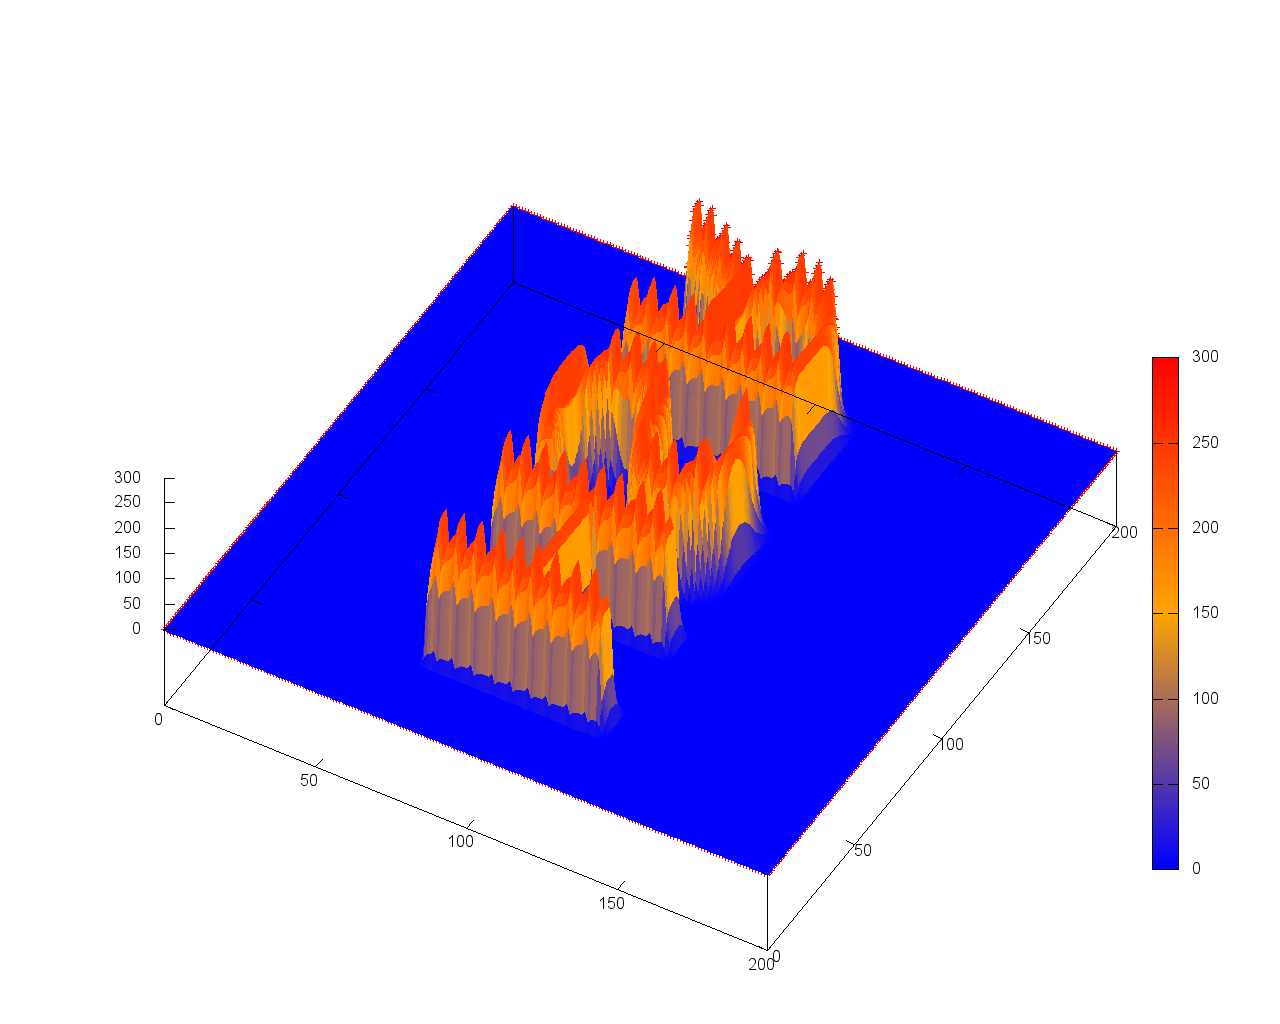
\includegraphics[width = 10cm]{../skript/images/step001}
\end{frame}